\section{Topology Skeletons}
Even though many algorithms can be expressed by parallel maps, some problems require more sophisticated skeletons. The Eden library leverages this problem and already comes with more predefined skeletons, among them the \code{pipe}, \code{ring} and a \code{torus} implementation \cite{eden_cefp, eden_skel_topology}. These seem like reasonable candidates to be ported to our arrow based parallel Haskell to prove that we can express such skeletons with Arrows as well.

\subsection{pipe}

\begin{lstlisting}[frame=htrbl]
pipe :: (ArrowLoop arr,
	ArrowParallel arr (fut a) (fut a) conf, Future fut a) =>
	conf -> [arr a a] -> arr a a
pipe conf fs = unliftFut (pipeFut conf fs)

pipeFut :: (ArrowLoop arr,
	ArrowParallel arr (fut a) (fut a) conf, Future fut a) =>
	conf -> [arr a a] -> arr (fut a) (fut a)
pipeFut conf fs =
	loop (arr snd &&& (arr (uncurry (:) >>> lazy) >>>
		parEvalNFut conf fs)) >>>
	arr last
\end{lstlisting}

\subsection{ring}

\begin{lstlisting}[frame=htrbl]
ring :: (ArrowLoop arr, Future fut r, ArrowParallel arr (i, fut r) (o, fut r) conf) =>
    conf ->
    arr (i, r) (o, r) ->
    arr [i] [o]
ring conf f =
	loop (second (rightRotate >>> lazy) >>>
    arr (uncurry zip) >>>
    parMap conf (second get >>> f >>> second put) >>>
    arr unzip)

-- from Eden, ported to Arrows:
rightRotate :: (Arrow arr) => arr [a] [a]
rightRotate = arr $ \list -> case
	list of [] -> []
			xs -> last xs : init xs
\end{lstlisting}

\subsection{torus}

\begin{lstlisting}[frame=htrbl]
torus :: (ArrowLoop arr, ArrowChoice arr, ArrowApply arr,
            ArrowParallel arr (c, fut [a], fut [b]) (d, fut [a], fut [b]) conf,
            Future fut [a], Future fut [b]) =>
         conf ->
         arr (c, [a], [b]) (d, [a], [b]) ->
         arr [[c]] [[d]]
torus conf f =
	loop (second ((mapArr rightRotate >>> lazy) ***
			(arr rightRotate >>> lazy)) >>>
    arr (uncurry3 (zipWith3 lazyzip3)) >>>
    (arr length >>> arr unshuffle) &&&
        (shuffle >>> parEvalN conf (repeat (ptorus f))) >>>
    app >>> arr (map unzip3) >>> arr unzip3 >>> threetotwo)

uncurry3 :: (a -> b -> c -> d) -> (a, (b, c)) -> d
uncurry3 f (a, (b, c)) = f a b c

lazyzip3 :: [a] -> [b] -> [c] -> [(a, b, c)]
lazyzip3 as bs cs = zip3 as (lazy bs) (lazy cs)

ptorus :: (Arrow arr, Future fut [a], Future fut [b]) =>
          arr (c, [a], [b]) (d, [a], [b]) ->
          arr (c, fut [a], fut [b]) (d, fut [a], fut [b])
ptorus f =
	arr (\ ~(c, fas, fbs) -> (c, get fas, get fbs)) >>>
	f >>>
	arr (\ ~(c, as, bs) -> (c, put as, put bs))

threetotwo :: (Arrow arr) => arr (a, b, c) (a, (b, c))
threetotwo = arr $ \ ~(a, b, c) -> (a, (b, c))
\end{lstlisting}

\begin{figure}[ht]
	\centering
	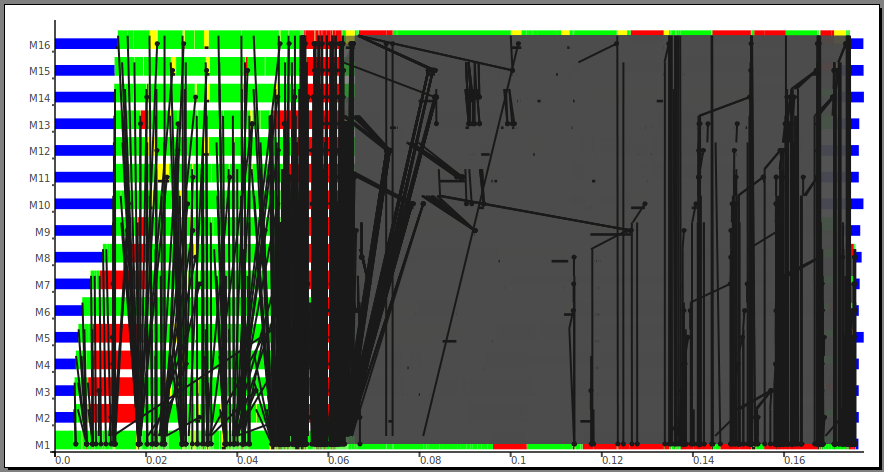
\includegraphics[width=0.9\textwidth]{images/torus_matrix_parrows}
	\caption[without Futures]{Matrix Multiplication with a torus (Parrows)}
\end{figure}

\begin{figure}[ht]
	\centering
	\includegraphics[width=0.9\textwidth]{images/torus_matrix_eden}
	\caption[with Futures]{Matrix Multiplication with a torus (Eden)}
\end{figure}